\begin{sol}[1](Résolu par Matthias Schuller)

On a $3^{2n}=9^n$,
or $9 \equiv 2 [7]$,
donc pour tout $n \in \mathbb{N}$, $9^n \equiv 2^n [7]$,
donc $3^{2n}-2^n \equiv 0 [7]$.

\end{sol}

\begin{sol}[29](Résolu par Sébastien Labbé)

Soit $s=min(x,\frac{1}{x}+y, \frac{1}{y})$.
Pour $x=\sqrt{2}$ et $\frac{1}{y}=\sqrt{2}$, on a $\frac{1}{x}+y=\sqrt{2}$, donc $s=\sqrt{2}$.\\
De plus, si $x\leq \sqrt{2}$ ou $\frac{1}{y} \leq \sqrt{2}$, on a $s \leq \sqrt{2}$.\\
Sinon, on a $x> \sqrt{2}$ et $\frac{1}{y}>\sqrt{2}$, on a $\frac{1}{x}+y<\sqrt{2}$, donc $s<\sqrt{2}$.\\
Ainsi la valeur maximale de $s$ vaut $\sqrt{2}$.


\end{sol}



\begin{sol}[34](Résolu par Rodion Zaystev)
On divise la figure

\[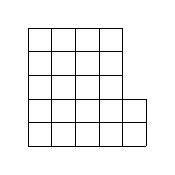
\begin{tikzpicture}[scale=0.3]
\draw (0, 0)--(0,5 );
\draw (1, 0)--(1,5 );
\draw (2, 0)--(2,5 );
\draw (3, 0)--(3,5 );
\draw (4, 0)--(4,5 );
\draw (5, 0)--(5,2 );

\draw(0,0)--(5,0);
\draw(0,1)--(5,1);
\draw(0,2)--(5,2);
\draw(0,3)--(4,3);
\draw(0,4)--(4,4);
\draw(0,5)--(4,5);
\end{tikzpicture}\]

en morceaux de forme 
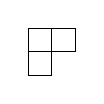
\begin{tikzpicture}[scale=0.3]
\draw(0,0)--(0,2);
\draw(1,0)--(1,2);
\draw(2,1)--(2,2);
\draw(0,0)--(1,0);
\draw(0,1)--(2,1);
\draw(0,2)--(2,2);
\end{tikzpicture}
et
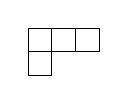
\begin{tikzpicture}[scale=0.3]
\draw(0,0)--(0,2);
\draw(1,0)--(1,2);
\draw(2,1)--(2,2);
\draw(3,1)--(3,2);
\draw(0,0)--(1,0);
\draw(0,1)--(3,1);
\draw(0,2)--(3,2);
\end{tikzpicture}.


Celle-ci est constituée de $22$ cases 
On note $x$ le nombre de morceaux de $3$ cases, et $y$ celui de ceux de $4$ cases.
On a alors $3x+4y=22$, et $x \geq 0$ et $y \geq 0$, donc $y \leq 5$.
Or $y$ est un entier, donc il n'y a que $6$ valeurs possibles de $y$:
\begin{itemize}
	\item[y=0:] Impossible car $3x=22$ avec $x$ entier
	\item[y=1:] $3x=18$ donc $x=6$
	\item[y=2:] Impossible car $3x=14$ avec $x$ entier
	\item[y=3:] Impossible car $3x=10$ avec $x$ entier
	\item[y=4:] $3x=6$ donc $x=2$
	\item[y=5:] Impossible car $3x=2$ avec $x$ entier
\end{itemize}
Ainsi les seules valeures possibles de $x$ sont $2$ et $6$.
Réciproquement, les deux figures suivantes montrent que ces $2$ valeurs conviennent effectivement.

\[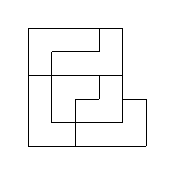
\begin{tikzpicture}[scale=0.3]
\draw (0, 0)--(0,5 );
\draw (1, 1)--(1,4 );
\draw (2, 0)--(2,2 );
\draw (3, 2)--(3,3 );
\draw (3, 4)--(3,5 );
\draw (4, 1)--(4,5 );
\draw (5, 0)--(5,2 );

\draw(0,0)--(5,0);
\draw(1,1)--(4,1);
\draw(2,2)--(3,2);
\draw(4,2)--(5,2);
\draw(0,3)--(4,3);
\draw(1,4)--(3,4);
\draw(0,5)--(4,5);
\end{tikzpicture}\]

\[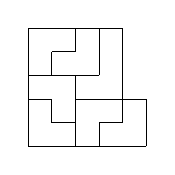
\begin{tikzpicture}[scale=0.3]
\draw (0, 0)--(0,5 );
\draw (1, 1)--(1,2 );
\draw (1, 3)--(1,4 );
\draw (2, 0)--(2,3 );
\draw (2, 4)--(2,5 );
\draw (3, 0)--(3,1 );
\draw (3, 3)--(3,5 );
\draw (4, 1)--(4,5 );
\draw (5, 0)--(5,2 );

\draw(0,0)--(5,0);
\draw(1,1)--(2,1);
\draw(3,1)--(4,1);
\draw(0,2)--(1,2);
\draw(2,2)--(5,2);
\draw(0,3)--(3,3);
\draw(1,4)--(2,4);
\draw(0,5)--(4,5);
\end{tikzpicture}\]

\end{sol}

\begin{sol}[42](Résolu par Maël Laoufi et Thibaut Desort)

Soit $x=1+\dfrac{1}{2+\dfrac{1}{2+\dfrac{1}{\cdots}}}$.

On remarque que $x=1+\dfrac{1}{1+1+\dfrac{1}{2+\dfrac{1}{\cdots}}}$, 
d'où 
\begin{eqnarray*}
x &=& 1+\frac{1}{1+x} \\
x-1 &=& \frac{1}{1+x}\\
(x+1)(x-1) &=& 1\\
x^2-1 &=& 1\\
x^2 &=& 2\\
\end{eqnarray*}

D'où $x=\sqrt{2}$ puisque $x$ est strictement positif.


\end{sol}


\begin{sol}[56](Résolu par Barthélémy Pelletier et Gaël Gallot)

Barthélémy Pelletier groupe B
Gaël Gallot groupe B

L'aire du carré est $a^2$.

L'aire du triangle est $\frac{\sqrt{3}}{4}b^2$.

On veut $a^2=\frac{\sqrt{3}}{4}b^2$, soit $a=\frac{\sqrt[4]{3}}{2}b$ car $a$ et $b$ sont strictement positifs.

Or $\frac{\sqrt[4]{3}}{2}$ est un nombre irrationnel.
Ainsi, si $b$ est rationnel, alors le produit $\frac{\sqrt[4]{3}}{2}b$ sera aussi irrationnel et $a$ sera irrationnel.

Par conséquent, $a$ et $b$ ne peuvent pas être tous les deux rationnels.

\end{sol}
\begin{sol}[75](Résolu par Dario Shariatan)

Déterminons d'abord de combien de manières différentes il est possible de carreler un rectangle de taille $2 \times n$ avec des carreaux incolores. Notons $F(n)$ ce nombre.

Pour les rectangles de taille $2 \times 1$ ou $2 \times 2$ on voit aisément que :
\begin{itemize}
\item Il n'y a qu'une seule façon de carreler le rectangle $2\times 1$
\item Il y a deux façons de carreler le rectangle $2 \times 2$ (carreaux horizontaux ou verticaux)
\end{itemize}

Pour carreler un carreau de taille $2 \times (n+1)$ il n'y a qu'une seule manière de s'y prendre :
\begin{itemize}
\item Soit on commence par un carreau $2 \times 1$ au début du rectangle et on carrele le rectangle de taille $2 \times (n-1)$ restant, il y a $F(n-1)$ possibilités
\item Soit on commence par deux carreaux $1 \times 2$ et on a $F(n-2)$ possibilités pour compléter le rectangle.
\end{itemize}

On a donc la relation de récurrence $F(n) = F(n-1) + F(n-2)$.

Étudions maintenant l'influence des couleurs. Pour carreler un rectangle, on utilise $n$ carreaux, qui peuvent chacun être colorés de deux manières différentes. Considérons un carrelage incolore donné, comme la position des carreaux est importante, il y a $2^n$ manières de colorier cette disposition. 

Ainsi, le nombre de manières de carreler un rectangle $2 \times n$ est $2^n \times F(n)$ où $F(n)$ est le $(n+1)$-ième terme de la suite de Fibonacci.

\end{solution}


\begin{sol}[130](Résolu par Pierre-Marie Esmenjaud Thibaut Maron)

Soit $a,b,c$ les longueurs des côtés d'un triangle. Montrons que l'on a toujours $a^2b(a-b)+b^2c(b-c)+c^2a(c-a) \geq 0$.\\
On utilise la substitution de Ravi, il existe $x,y,z$ positifs tels que 
$a=x+y$,$b=y+z$, $c=z+x$.
En développant l'inégalité et en la simplifiant, on obtient alors
$2(x^3y+y^3x+z^3y-x^2yz-y^2xz-z^2xy) \geq 0$,
c'est-\`a-dire $x^3y+y^3x+z^3y \geq x^2yz+y^2xz+z^2xy$
Or les suites $(x^2,y^2,z^2)$ et $(yz,xz,xy)$ sont dans l'ordre opposé, donc par l'in\'egalit\'e de r\'eordonnement,
on a $x^2xy+y^2yz+z^2zy \geq x^2yz+y^2xz+z^2xy$, ce qui correspond \`a l'in\'egalit\'e initiale.

\end{sol}

\begin{sol}[130](Résolu par Paul Rax)

Supposons par l'absurde qu'il existe une suite $(u_n)_{n \in \mathbb{N}^*}$ telle que pour tout $n,m \in \mathbb{N}^*$, on ait
$u_{nm}=u_n+u_m$. Prenons le $2u_3$-i\`eme \'el\'ement. On a alors $u_{2u_3}=u_2+u_{u_3}$.\\
Par ailleurs, la suite est une suite d'entiers strictement croissante, et $u_{2u_3}$ et $u_{u_3}$ sont s\'epar\'es de $u_3$ rangs,
donc on a $u_{2u_3} \geq u_{u_3} +u_3$, donc $u_2+u_{u_3} \geq u_{u_3} +u_3$, donc $u_2 \geq u_3$, ce qui contredit la stricte croissance de la suite.\\
Ainsi il n'existe pas de telle suite.

\end{sol}



\begin{sol}[99](Résolu par Baptiste Serraille)

		\definecolor{uuuuuu}{rgb}{0.26666666666666666,0.26666666666666666,0.26666666666666666}
		\definecolor{qqqqff}{rgb}{0.,0.,1.}
		\begin{center}
		\begin{tikzpicture}[line cap=round,line join=round,>=triangle 45,x=0.5cm,y=0.5cm]
		\clip(-4.8866410764292,-5.572904036609516) rectangle (24.92335892357077,7.055095963390474);
		\draw (3.38,4.66)-- (4.6,-3.1);
		\draw (4.6,-3.1)-- (13.6,-3.2);
		\draw (3.38,4.66)-- (13.6,-3.2);
		\draw(6.6073797978803945,-0.7786041073342618) circle (1.171777726594992cm);
		\draw (3.8617737962416823,1.595602738659465)-- (7.415842784909827,1.556113083229819);
		\draw (1.0600044164045799,-3.0606667157378284)-- (5.638808290575755,1.575857910944642);
		\draw (1.0600044164045799,-3.0606667157378284)-- (6.581341825154507,-3.1220149091683833);
		\draw (1.0600044164045799,-3.0606667157378284)-- (8.036095081092272,1.0790893016257088);
		\begin{scriptsize}
		\draw [color=qqqqff] (3.38,4.66)-- ++(-2.5pt,-2.5pt) -- ++(5.0pt,5.0pt) ++(-5.0pt,0) -- ++(5.0pt,-5.0pt);
		\draw[color=qqqqff] (3.5393589235707914,5.053095963390476) node {$A$};
		\draw [color=qqqqff] (4.6,-3.1)-- ++(-2.5pt,-2.5pt) -- ++(5.0pt,5.0pt) ++(-5.0pt,0) -- ++(5.0pt,-5.0pt);
		\draw[color=qqqqff] (4.199358923570791,-2.712904036609518) node {$B$};
		\draw [color=qqqqff] (13.6,-3.2)-- ++(-2.5pt,-2.5pt) -- ++(5.0pt,5.0pt) ++(-5.0pt,0) -- ++(5.0pt,-5.0pt);
		\draw[color=qqqqff] (13.747358923570783,-2.800904036609518) node {$C$};
		\draw [color=uuuuuu] (8.036095081092272,1.0790893016257088)-- ++(-2.5pt,-2.5pt) -- ++(5.0pt,5.0pt) ++(-5.0pt,0) -- ++(5.0pt,-5.0pt);
		\draw[color=uuuuuu] (8.445358923570787,1.3350959633904789) node {$E$};
		\draw [color=uuuuuu] (4.292261123652807,-1.1425789504473618)-- ++(-2.5pt,-2.5pt) -- ++(5.0pt,5.0pt) ++(-5.0pt,0) -- ++(5.0pt,-5.0pt);
		\draw[color=uuuuuu] (3.913358923570791,-0.9309040366095195) node {$F$};
		\draw [color=uuuuuu] (6.581341825154507,-3.1220149091683833)-- ++(-2.5pt,-2.5pt) -- ++(5.0pt,5.0pt) ++(-5.0pt,0) -- ++(5.0pt,-5.0pt);
		\draw[color=uuuuuu] (6.729358923570788,-2.734904036609518) node {$D$};
		\draw [color=uuuuuu] (1.0600044164045799,-3.0606667157378284)-- ++(-2.5pt,-2.5pt) -- ++(5.0pt,5.0pt) ++(-5.0pt,0) -- ++(5.0pt,-5.0pt);
		\draw[color=uuuuuu] (0.7233589235707943,-2.690904036609518) node {$T$};
		\draw [color=uuuuuu] (6.6334177706062825,1.5648066944998584)-- ++(-2.5pt,-2.5pt) -- ++(5.0pt,5.0pt) ++(-5.0pt,0) -- ++(5.0pt,-5.0pt);
		\draw [color=uuuuuu] (3.8617737962416823,1.595602738659465)-- ++(-2.5pt,-2.5pt) -- ++(5.0pt,5.0pt) ++(-5.0pt,0) -- ++(5.0pt,-5.0pt);
		\draw[color=uuuuuu] (4.023358923570791,1.9950959633904781) node {$H$};
		\draw [color=uuuuuu] (7.415842784909827,1.556113083229819)-- ++(-2.5pt,-2.5pt) -- ++(5.0pt,5.0pt) ++(-5.0pt,0) -- ++(5.0pt,-5.0pt);
		\draw[color=uuuuuu] (7.719358923570788,2.1930959633904776) node {$G$};
		\draw [color=uuuuuu] (5.638808290575755,1.575857910944642)-- ++(-2.5pt,-2.5pt) -- ++(5.0pt,5.0pt) ++(-5.0pt,0) -- ++(5.0pt,-5.0pt);
		\draw[color=uuuuuu] (5.783358923570789,1.9730959633904783) node {$M$};
		\draw [color=uuuuuu] (4.939888935469334,0.8681279248895978)-- ++(-2.5pt,-2.5pt) -- ++(5.0pt,5.0pt) ++(-5.0pt,0) -- ++(5.0pt,-5.0pt);
		\draw[color=uuuuuu] (4.595358923570791,1.3790959633904787) node {$T_1$};
		\end{scriptsize}
		\end{tikzpicture}
		\end{center}			
		La solution utilise deux résultats de géométrie projective avancés : 
		
		i) Pour un point et un cercle donnés, les deux points de contact avec les tangentes par ce point et deux points sur une sécantes sont en division harmonique
		
		ii) Le birapport de quatre points sur un cercle est égal au birapport des tangentes en ces points
		
		iii) Soient $A,B$ des points et $M$ le milieu de $[AB]$. Alors $A,B,M,\infty$ sont harmoniques. Réciproquement, si $A,B,M,\infty$ sont harmoniques, alors $M$ le milieu de $[AB]$.
		
		Début de la solution :
		
		Soit $T_1$ le point de contact de la tangente (autre que $(TC)$) au cercle inscrit. Et soit $M_1$ le point d'intersection de $TT_1$ avec $(GH)$. Montrons que $M_1$ est le mileu de $(GH)$.
				
		D'après i) $T_1 F E D$ sont en division harmonique
		
		D'après ii) $$-1 =b_{T_1,D,F,E}=b_{T_1M_1,DB,FH,EG}=b_{M_1,\infty,H,G}$$
		
		Donc, d'après iii), $M_1$ est bien le milieu de $[HG]$.
\end{sol}

\begin{sol}[130](Résolu par Thibaut Maron)

Soit $x_1,x_2,\dots,x_{13}$ $13$ r\'eels deux \`a deux distincts.\\
La fonction tangente réalise une surjection (en fait une bijection) de $]-\frac{\pi}{2},\frac{\pi}{2}[$ dans $\mathbb{R}$, donc il existe $13$ réels $a_1,a_2,\dots,a_{13}$ appartenant tous \`a $]-\frac{\pi}{2},\frac{\pi}{2}[$ (intervalle de largeur $\pi$),
vérifiant $\forall i \in [[1,13]], \tan(a_i)=x_i$. \\
Or, par le principe des tiroirs, il existe $i$ et $j$ distincts tels que $ 0 \leq a_i-a_j \leq \frac{\pi}{12}$
Or la fonction tangente est croissante sur $]-\frac{\pi}{2},\frac{\pi}{2}[$, donc on peut composer l'in\'egalit\'e pr\'ec\'edente par tangente, \\
on obtient ainsi $\tan(0) \leq \tan(a_i-a_j) \leq \tan(\frac{\pi}{12})$, \\
en appliquant une formule de trigonométrie, \\
on a donc $0 \leq \frac{\tan(a_i)-\tan(a_j)}{1+\tan(a_i)\tan(a_j)} \leq 2-\sqrt{3} $ \\
Or $\forall i \in [[1,13]], \tan(a_i)=x_i$, \\
ainsi $0 \leq \frac{x_i-x_j}{1+x_i x_j} \leq 2-\sqrt{3}$,
ce qui conclut.
\end{sol}

\begin{sol}[59](R\'esolu par Th\'eodore Fougereux et Timoth\'ee Roquet)

		Soit, pour $0 < x < \frac{\pi}{2}$, $f(x)=\left(1+\frac{1}{(\cos x)^{10}}\right)\left(1+\frac{1}{(\sin x)^{10}}\right)$.
		$f$ est d\'erivable et sa d\'eriv\'ee est \\ $f':~x \longmapsto \frac{10\sin(x)}{(\cos(x))^{11}}\left(1+\frac{1}{(\sin(x))^{10}}\right) - \frac{10 \cos(x)}{(\sin(x))^{11}}\left(1+\frac{1}{(\cos(x))^{10}}\right)$. \\
		Si $0 < x < \frac{\pi}{2}$, $f'(x) = \frac{10}{(\sin(x))^{11}(\cos(x))^{11}}\left((\sin(x))^{12}+(\sin(x))^2 - ((\cos(x))^{12}+(\cos(x))^2)\right)$, donc $f'(x)$ a le signe de $g(\sin(x))-g(\cos(x))$, o\`u $g:~x \longmapsto x^{12}+x^2$ qui est strictement croissante sur $\mathbb{R}^+$, et par cons\'equent $f$ d\'ecro\^it avant $\frac{\pi}{4}$ et cro\^it apr\`es. Par cons\'equent, $f$ est minimale en $\frac{\pi}{4}$ et on calcule $f\left(\frac{\pi}{4}\right)=1089$, ce qui conclut.\\
		
		\textit{Une autre preuve est possible}: pour $x > 0$, on note $f(x)=\ln\left(1+\frac{1}{x^5}\right)$, $f$ est d\'erivable et pour $x > 0$, $f'(x)=\frac{\frac{-5}{x^6}}{1+\frac{1}{x^5}}=\frac{-5}{x^6+x}$, et en cons\'equence $f'$ est croissante, donc $f$ est convexe. On a, pour $0 < x < \frac{\pi}{2}$, 
		\[\ln\left(\left(1+\frac{1}{(\cos(x))^{10}}\right)\left(1+\frac{1}{(\sin(x))^{10}}\right)\right) = f((\cos(x))^2)+f((\cos(x))^2) \geq 2f\left(\frac{(\cos(x))^2+(\sin (x))^2}{2}\right) = 2 \ln(33) = \ln (1089).\]
\end{sol}

\begin{sol}[64](R\'esolu par Humbert Tristan)

		Si $p!^k | (p^2)!$, $k*v_p(p!) = v_p(p!^k) \leq v_p((p^2)!)$. 
		Or, la formule de Legendre donne $v_p(p!)=p$, et $v_p((p^2)!)=p+1$. En cons\'equence, si $p!^k | p^2!$, $k \leq p+1$. \\
		On va montrer que $p!^{p+1} | p^2!$. Soit $q$ un premier divisant $p!$ et distinct de $p$ (le r\'esultat du paragraphe est, on l'a vu, vrai pour $p$), soit $i \in \N$, \'ecrivons $p=q^i*a+r$, avec $0 \leq r < q^i$, et $a,r$ entiers. Par primalit\'e de $p$, $r > 0$, on a alors \\ $\left\lfloor \frac{p^2}{q^i}\right\rfloor = \left\lfloor \frac{a^2q^{2i}+2arq^i+r^2}{q^i}\right\rfloor=a^2q^i+2ar+\left\lfloor \frac{r^2}{q^i}\right\rfloor \geq a(aq^i+r+r) \geq (p+1) \left\lfloor \frac{p}{q^i}\right\rfloor$. En sommant, on obtient, pour tout premier $q < p$, $(p+1)v_q(p!) \leq v_q(p^2!)$. \\
		On a alors $p!^{p+1} | p^2!$, et tel n'est pas le cas pour $p!^{p+2}$. 
\end{sol}

\begin{sol}[126](Résolu par Joachim Studnia)

Notons $p=3k+2$ avec $p$ premier divisant $a^2+ab+b^2$. Supposons par l'absurde que $p$ ne divise pas $a$. Alors clairement $p$ ne divise pas $b$.

$a^3-b^3 = (a-b)(a^2+ab+b^2)$ donc $p | a^3-b^3$ et $a^3 \equiv b^3 \pmod p$ (I).

D'après le petit théorème de Fermat, \mbox{$a^{p-1} \equiv b^{p-1} \equiv 1 \pmod p$}, d'où \mbox{$a^{3k+1} \equiv b^{3k+1} \pmod p$}. (II)

D'après (I), $a^{3k} \equiv b^{3k} \pmod p$ donc $(a^{3k})^{-1} \equiv (b^{3k})^{-1} \pmod p$, c'est-à-dire $a^{-3k} \equiv b^{-3k} \pmod p$.

D'après (II), on en déduit que $a \equiv b \pmod p$, donc \mbox{$a^2+ab+b^2 \equiv 3a^2 \pmod p$}.

On a donc $p | 3a^2$ par hypothèse, donc soit $p | 3$, ce qui est exclu car \mbox{$p \equiv 2 \pmod 3$}, soit $p |a$, ce qui est en contradiction avec l'hypothèse de départ.

Ainsi, $p$ divise $a$ et $b$.

\end{sol}

\begin{sol}[133](Résolu par Yakob Kahane)

		Si on a deux points sur un cercle, alors le centre dudit cercle se trouve sur la m\'ediatrice des deux points. Si lesdits deux points sont \`a coordonn\'ees rationnelles, leur m\'ediatrice poss\`ede une \'equation \`a coefficients rationnels. \\
			On suppose d\`es lors qu'il existe $A$, $B$, $C$ trois points \`a coordonn\'ees rationnelles sur un m\^eme cercle $\Gamma$ dont le centre n'est pas \`a coordonn\'ees rationnelles. On note $L_1$, $L_2$ des \'equations respectives des m\'ediatrices de $[AB]$ et $[AC]$ \`a coefficients rationnels:
			\[L_1: a_1x+b_1y=c_1\]
			\[L_2: a_2x+b_2y=c_2\]
			Leur point d'intersection est la solution d'un syst\`eme de deux \'equations \`a deux inconnues \`a coefficients rationnels; le calcul de la solution (ie du point d'intersection) se fait en restant dans $\Q$; or ce point $O$ d'intersection est le centre d'un cercle circonscrit \`a $ABC$ donc de $\Gamma$, ce qui contredit l'hypoth\`ese. \\
			Il reste \`a trouver deux points rationnels sur un cercle de centre de coordonn\'ees irrationnelles. Le lecteur v\'erifiera qu'un cercle de centre $O(\sqrt{2};1-\sqrt{2})$ passe par $A(0;0)$ et $B(1;1)$,ce qui conclut.  
\end{sol}

\begin{sol}[13](R\'esolu par Jules Bouton)

		\definecolor{uuuuuu}{rgb}{0.26666666666666666,0.26666666666666666,0.26666666666666666}
\definecolor{zzttqq}{rgb}{0.6,0.2,0.}
\definecolor{qqqqff}{rgb}{0.,0.,1.}
\begin{tikzpicture}[line cap=round,line join=round,>=triangle 45,x=1.0cm,y=1.0cm]
\clip(-4.3,-2.56) rectangle (7.06,6.3);
\fill[color=zzttqq,fill=zzttqq,fill opacity=0.1] (-0.78,2.78) -- (3.64,-0.96) -- (-2.06,-1.18) -- cycle;
\draw [color=zzttqq] (-0.78,2.78)-- (3.64,-0.96);
\draw [color=zzttqq] (3.64,-0.96)-- (-2.06,-1.18);
\draw [color=zzttqq] (-2.06,-1.18)-- (-0.78,2.78);
\draw [domain=-2.06:7.0600000000000005] plot(\x,{(--1.6788--2.9*\x)/3.64});
\begin{scriptsize}
\draw [fill=qqqqff] (-0.78,2.78) circle (2.5pt);
\draw[color=qqqqff] (-0.64,3.14) node {$A$};
\draw [fill=qqqqff] (3.64,-0.96) circle (2.5pt);
\draw[color=qqqqff] (3.78,-0.6) node {$B$};
\draw [fill=qqqqff] (-2.06,-1.18) circle (2.5pt);
\draw[color=qqqqff] (-1.92,-0.82) node {$C$};
\draw [fill=uuuuuu] (1.0096989966555185,1.2656393105222536) circle (1.5pt);
\draw[color=uuuuuu] (1.14,1.54) node {$I$};
\end{scriptsize}
\end{tikzpicture}

		\begin{itemize}
				\item[$\Rightarrow$] La loi des sinus donne $\frac{AI}{\sin(\widehat{ACI})}=\frac{AC}{\sin(\widehat{AIC})}$ et $\frac{BI}{\sin(\widehat{ICB})}=\frac{BC}{\sin(\widehat{CIB})}$, ce qui donne $\frac{AI}{AC}=\frac{\sin(\widehat{ACI})}{\sin(\widehat{AIC})}$ et $\frac{BI}{BC}=\frac{\sin(\widehat{ICB})}{\sin(\widehat{CIB})}$. Comme $\widehat{AIC}$ et $\widehat{CIB}$ sont suppl\'ementaires, ils ont m\^eme sinus. Comme $\widehat{ACI}=\widehat{ICB}$ par hypoth\`ese, on d\'eduit$\frac{BI}{BC}=\frac{AI}{AC}$, c'est-\`a-dire $\frac{CB}{CA}=\frac{IB}{IA}$. \\
				\item[$\Leftarrow$] La loi des sinus donne $\frac{AI}{\sin(\widehat{ACI})}=\frac{AC}{\sin(\widehat{AIC})}$ et $\frac{BI}{\sin(\widehat{ICB})}=\frac{BC}{\sin(\widehat{CIB})}$, ce qui donne $\frac{AI}{AC}=\frac{\sin(\widehat{ACI})}{\sin(\widehat{AIC})}$ et $\frac{BI}{BC}=\frac{\sin(\widehat{ICB})}{\sin(\widehat{CIB})}$. De $\frac{CA}{CB} = \frac{IA}{IB}$ vient $\frac{AI}{AC}=\frac{BI}{BC}$, et en cons\'equence $\frac{\sin(\widehat{ACI})}{\sin(\widehat{AIC})}=\frac{\sin(\widehat{BCI})}{\sin(\widehat{BIC})}$. Comme $\widehat{ACI}$ et $\widehat{BIC}$ sont suppl\'ementaires, ils ont m\^eme sinus.
				On d\'eduit \\ $\sin(\widehat{ACI})=\sin(\widehat{ICB})$, donc les deux angles sont \'egaux (ils ne peuvent pas \^etre suppl\'ementaires) et $(CI)$ est la bissectrice int\'erieure de $\widehat{ACB}$. 
		\end{itemize}~\\
		\textit{On peut aussi prouver le r\'esultat comme suit:} soient $ABC$ un triangle acutangle, $I$ un point du segment $[AB]$, $a = \frac{AI}{AC}$, $b = \frac{BI}{BC}$. De la loi des sinus on d\'eduit $\frac{AI}{\sin(\widehat{ACI})}=\frac{AC}{\sin(\widehat{AIC})}$ et \\ $\frac{BI}{\sin(\widehat{ICB})}=\frac{BC}{\sin(\widehat{CIB})}$, c'est-\`a-dire $a = \frac{\sin(\widehat{ACI})}{\sin(\widehat{AIC})}$ et $b=\frac{\sin(\widehat{BCI})}{\sin(\widehat{BIC})}$. Comme $\widehat{ACI}$ et $\widehat{BIC}$ sont suppl\'ementaires, ils ont m\^eme sinus, d'o\`u $\frac{b}{a}=\frac{\sin(\widehat{ACI})}{\sin(\widehat{ICB})}$. \\
		Finalement, $\frac{CA}{CB}=\frac{IA}{IB} \Leftrightarrow a = b \Leftrightarrow \widehat{ACI}=\widehat{ICB}$, le dernier point \'etant \'equivalent \`a "$(CI)$ est la bissectrice int\'erieure de $\widehat{ACB}$"'.
\end{sol}

\begin{sol}[1](Résolu par ....)

Lorem Ipsum

\end{sol}
